\documentclass[smallextended,natbib]{svjour3}

%%% custom 

\newcommand{\beqa}{\begin{eqnarray}}
\newcommand{\beq}{\begin{equation}}
\newcommand{\eeqa}{\end{eqnarray}}
\newcommand{\eeq}{\end{equation}}


\usepackage{amsmath,amssymb}
\usepackage{natbib}
\usepackage{nameref,hyperref}
\newcommand{\micron}{\mu\textrm{m}}
\newcommand{\norm}[1]{\left|\left|#1\right|\right|}

\usepackage{color}
\newcommand{\red}[1]{\textcolor{red}{#1}}

\newcommand{\hatvec}[1]{\hat{\vec{#1}}}

\newcommand{\oxy}{\mathrm{pO}_2}
\newcommand{\braces}[1]{\left\{#1\right\}}

\bibliographystyle{plainnat}

\usepackage{graphicx}
\usepackage{epstopdf}

\begin{document}

\title{Computational multicellular systems biology in cancer:}
% Multiscale biophysics simulations of the liver:}
% Multiscale biophysics of colon cancer liver metastases: }
\subtitle{Simulating the impact of parenchymal fluid flow and tissue mechanics on colon cancer metastases of 
the liver\footnote{Better titles appreciated}}
\dedication{Dedicated to all the papers we should have written.}

\author{Paul Macklin${}^{*,\dagger}$\thanks{${}^{*}$ Invited and corresponding author}\thanks{${}^{\dagger}$ Contributed equally to this work} \and Jessica Sparks${}^{\dagger}$ \and Hermann B. Frieboes  
\and Erik Brodin 
\and Ahmadreza Ghaffarizadeh  \and Shannon M. Mumenthaler}
\institute{P. Macklin \and A. Ghaffarizadeh \and S.M. Mumenthaler 
\at Lawrence J. Ellison Institute for Transformative Medicine, University of Southern California, 
2250 Alcazar St., CSC-248, Los Angeles, CA 90033, USA\\Tel.: 310-701-5785, \email{Paul.Macklin@MathCancer.org}, www: \url{http://MathCancer.org}
H.B. Frieboes \at DEPARTMENT, University of Louisville, ADDRESS, Louisville, KY ZIP, USA 
\and 
J. Sparks \and E. Brodin \at 
Dept. of Chemical, Paper and Biomedical Engineering, Miami Univiersity, (address), Oxford, OH ZIP, USA}

\titlerunning{Short title}
\authorrunning{Macklin et al.}

\maketitle


\begin{abstract}150-250 words
This is an awesome paper! 
This is an awesome paper! 
This is an awesome paper! 
This is an awesome paper! 
This is an awesome paper! 
This is an awesome paper! 
This is an awesome paper! 
This is an awesome paper! 
This is an awesome paper! 
This is an awesome paper! 
This is an awesome paper! 
This is an awesome paper! 
This is an awesome paper! 
This is an awesome paper! 
This is an awesome paper! 
This is an awesome paper! 
This is an awesome paper! 
This is an awesome paper! 
This is an awesome paper! 
This is an awesome paper! 
This is an awesome paper! 
This is an awesome paper! 
This is an awesome paper! 
This is an awesome paper! 
This is an awesome paper! 
This is an awesome paper! 
This is an awesome paper! 
This is an awesome paper! 
\keywords{Neat \and Cool}
\subclass{MSC codes}
\PACS{PACS codes}
\CRclass{CR codes}
\end{abstract}

\section{Introduction}
\red{Paul, Jessica, and Shannon write.}
%Colon cancer mets in liver are bad.  
%Prognosis known to be TME-dependent. 
%Impact of parenchymal mechanics and flow on growth poorly understood, as is the biology regulationg tumor-parenchyme 
%interactions at the tumor boundary.  
%New emerging experimetnal platforms allow probing these dynamics, but still difficult to measure flow dynamics at 
%small scales, in and around tumor foci. Modeling can help. 
Different models give different insights. We are working to integrate these insights. 
Continuum model helps motivate discrete model. 
Discrete model helps motivate continuum model. 
Part of a larger-scale effort to dynamically link codes, create open source framework 
for experimentally-driven multicellualr systems biology.  \red{Paul}

\begin{enumerate}
\item 
Colon cancer metastasizes to the liver. big clinical problem. bad.  \red{Jessica, Shannon}
\item 
Impact of TME unknown, but does impact prognosis \red{Jessica, Shannon}
\item 
Impact of parenchymal mechanics and flow on growth poorly understood, as is the biology regulating tumor-parenchyme interactions 
at the tumor boundary. \red{Jessica, Shannon}
\item 
New emerging platforms allow you to directly problem some dynamics, but can't measure everything. Difficult ot measure flow dynamics at 
small scales, in and aroudn foci. Modeling can help.  \red{Jessica, Shannon}
\item 
open questions: 
\begin{enumerate}
\item 
Where do mets most commonly seed? \red{Jessica, Shannon}
\item
How do they alter mechanics adn flow of the liver? \red{Jessica, Hermann}
\item 
How do cancer cells impact surrounding hepatocytes? \red{Jessica, Shannon}
\item 
Tumor cells are often densely packed, but lower cell-cell adhesion? So, is relative permeability higher or lower? Impact on growth 
dynamics? \red{Jessica, Paul, Hermann}
\end{enumerate}
\item 
math modeling is a way to fill in the missing pieces, generate testable hypotheses. \red{Paul, Jessica, Hermann}
\item 
Give flavor of past modeling results. Note that most is tissue regeneration, toxicology, or single-scale models of flow.  
\red{Paul, Jessica, Hermann}
\item 
And now the fun twist: in most multiscale investigations, discrete or smaller-scale simulations are used to generate insights for 
larger-scale continuum models. Here, we do the opposite: use a very detailed continuum model of flow, mechanics to generate insights 
to build a discrete multicellular model. \red{Paul}
\end{enumerate}


\begin{figure}\sidecaption 
% \resizebox{0.3\hsize}{!}{\includegraphics*{./figures/figure.eps}}
% \includegraphics*{./figures/figure.eps}
\caption{Overall schematic of trading insights between models.}
\label{fig:multiscale_models}
\end{figure}


% \citet{ghaffarizadeh15_bioinformatics} is a great paper \citep{ghaffarizadeh15_bioinformatics}. 

\subsection{Background biology \red{Shannon}}
Describe backround biology of liver (structurally: lobules with outflow from portal triads through parenchyma (sinusoids -- cords of heaptocytes surrounding channels, or sinusoids that are lined by thin, fenestratedendothelial cells), flowing out through central veins). Main role: metabolize toxins, act as a giant reactive blood sponge. :-) Also creates bile, but not main focus here.  
See Fig. \ref{fig:liver_schematic}. 

Anything else on the environment. General mechanics? General oxygenation? 

Then, the background of colon cancer mets. A preferred site for colon cancer metastases. Properties of most incomign cells. Things like this. 

Anything that Shannon things belongs here! 
% \cite{ghaffarizadeh15_bioinformatics} 

\begin{figure}[tbh]
Figure: overall liver geometry. 
\caption{Main organization of liver tissue} 
\label{fig:liver_schematic}
\end{figure}

\subsection{Prior modeling works \red{Jessica, Paul,Hermann}}
Describe past modeling efforts, limite insights, still not enough for CRC mets. Prior modeling restricted to colon cancer mets in 
liver, and potentially relevant liver models (most of which are focused on tissue engineering, healing, toxicology) \red{Paul, Jessica,Hermann}


Short literature review on prior models of liver flow, mechanics. 
Note much focused on PKPD, toxicity, strong work by Glazier group. 
Note much work on regeneration, strong work by Drasdo group. 
Others on flow. 
Little integration of these works. 
Pull from our NSF proposal. \red{Paul, Jessica,Hermann}

% \section{Method \red{Jessica, Paul}}

\subsection{Overall approach \red{Paul}}
We willl investigate using two modeling approaches. First, in Section 
\ref{section:PVE} we will use the PVE model to udnerstand flow, 
mechanics across a typical lobule, and to generate more insights on 
the fluid / mechanical state of the liver environment surrounding 
small tumor foci. 

In Section \ref{section:ABM}, we will use agent-based model 
to investigate cell and tisue biomechanics, transport-limited 
growth, and tumor-parenchymal interactions on growing tumor foci. 
Work will direclty incorporate insights from PVE. 


\section{First approach: Poroviscoelastic (PVE) model \red{Jessica}}
\label{section:PVE}
Short intro. 1 paragraph at most. 

\subsection{Method}
\subsection{Results}

\vfill
\pagebreak

\section{Second approach: Agent-based (PhysiCell) model \red{Paul,Hermann}}
\label{section:ABM}
\red{Short intro. 1 pararaph at most.  Note difficulty of adding interstitial flow at this scale. 
Kasia Rejnia did it with IBcell, but very small domains. Hermann did it in continuum tumor growth 
model. Jessica did it above in static tumor models. We're doing first-of-its-kind 1 cm2 
simulations, hundreds of lobules. So, we use insights from above to come up wtih good approximation. }

\subsection{Method} 
Describe the model of several liver lobules.  Include overall geometry, 
% We will seed the liver radially from portal triads, fill liver sinusoids with parenchyme cells, 
% empty to central vein. 

overall approach:
\begin{enumerate}
\item  
Model flow as quasi-steady, due to fast time scale 
\item 
Approximate flow as radially symmetric profile in each liver lobules, and extrapolate out to liver boundaries
\item 
Assume biotransport is 
\end{enumerate}

blah 

\subsubsection{Generating large 2-D liver tissues}
\label{sec:generate_liver}
To generate a large liver tissue, we (1) 
randomly place central veins (CVs) across the tissue, with  
mean density $\sim 2 \times 10^{-6} \micron^{-2}$ 
(to ensure a mean hepatic lobular diameter 
of 800 $\micron$); (2) replace any closely-spaced pairs of CVs with a 
single CV placed at their midpoint; and (3) we fill the remaining space 
with parenchymal agents. In this paper, we generated a 1 cm$^2$ liver 
tissue containing \red{?} hepatic lobules. See Fig. \ref{?} 

We have included a MATLAB script in the supplementary materials 
to implement this algorithm. It has the random seed hard-coded 
to reproduce the liver tissue used in this manuscript. 

\subsubsection{Integrating PVE insights: biotransport in unobstructed liver tissue}
We model biotransport in the liver tissue based upon the 
insights gained from the PVE model; see Section \ref{?}. In 
regions not occupied by tumor tissue, we assume that hepatic blood 
and interstitial flow are intact. (Hereafter, we 
refer to hepatic blood and interstitial flow collectively 
as ``flow'' for simplicity.) Moreover, we can assume that 
on the time scale of tissue mechanics (minutes to hours) and 
tumor cell proliferation (hours, days, and weeks), that flow occurs 
on a much faster time scale (seconds), and so biotransport is at quasi-steady 
state. Moreover, we will approximate flow as radially-symmetric in lobules not 
obstructed by tumor. Thus, we approximate $\vec{u} = - u(r) \hatvec{r}$, 
where $\hatvec{r}$ is the radial unit vector (oriented outward from the nearest
central vein), and $u(r)$ is the non-negative radial speed profile. 

We model the transport of a single growth substrate $\sigma$ 
(e.g., oxygen or glucose) in the tissue with 
\beqa
\frac{ \partial \sigma }{\partial t} & = & 
-\nabla \cdot \vec{J} - \lambda \sigma \label{eqn:transport1}  \\
\vec{J} &  = & -D \nabla \sigma + \sigma \vec{u} \label{eqn:transport2} , 
\eeqa
where $\vec{J}$ is the growth substrate flux, $\lambda$ is its 
consumption rate, and $D$ is its diffusion coefficient, which 
we assume is constant. 

To understand the relative contribution of the diffusional 
term in unobstructed flow, we nondimensionalize space with scale $L$, time 
with scale $\bar{t}$, and the flow with typical magnitude  
$\bar{u}$. With these scales, 
Equations \ref{eqn:transport1}-\ref{eqn:transport2} 
become 
\beq
\frac{ \partial  \sigma}{\partial t}  =  
\left( \frac{ D \bar t}{ L^2 } \right) \nabla^2 \sigma  
- \left(  \frac{\bar{u} \bar{t} }{L} \right)
\nabla \cdot \left( \sigma \vec{u} \right) 
 - \left( \lambda \bar{t} \right) \sigma. 
\eeq
Choosing 
\beq
\frac{ u \bar{t}}{L } = 1 \textrm{ and } \lambda \bar{t} = 1 
\Longrightarrow \bar{t} = \frac{1}{\lambda} \textrm{ and } 
L = \frac{ u }{ \lambda }, 
\eeq
then the nondimensionalized equation becomes 
\beq
\frac{ \partial  \sigma}{\partial t}  =  
\left( \frac{ D \lambda }{ \bar{u}^2 } \right) \nabla^2 \sigma  
- \nabla \cdot \left( \sigma \vec{u} \right) - \sigma . 
\eeq

By \citep{ghaffarizadeh15_bioinformatics}, 
$D \sim 10^5 \micron^2 / \textrm{min}$ and 
$\lambda \sim 10 \textrm{ min}^{-1}$. 
By the PVE work in Section \ref{?} and \citep{nishii}, 
$\bar{u} \sim 10^{-4} \textrm{m}/\textrm{sec} 
\sim 10^4 \:\micron/\textrm{min}$.  
% Note that $\bar{t} \sim 0.1 \textrm{ min}$
% = 6 \times 10^3 \micron/\textrm{min} 
% \sim 10^4 \:\micron/\textrm{min}$), 
% and so 
% $L \sim 600\:\micron$, 
% $\bar{t} \sim 6 \textrm{ sec}$. 
The diffusion term has relative order of magnitude 
\beq
\frac{ D \lambda }{ \bar{u}^2}  \sim 10^{-2}. 
\eeq
Thus, in unobstructed regions of liver lobule, flow is primarily advective-reactive, and we can simplify the original equation  to 
\beq
\frac{ \partial \sigma }{ \partial t} = -\nabla \cdot \left( \sigma \vec{u} \right) - \lambda \sigma. 
\eeq
Next, assuming incompressible flow ($\nabla \cdot \vec{u} = 0$) and 
that $\vec{u} \approx - u(r) \hatvec{r}$, we have 
\beqa
\frac{\partial \sigma}{\partial t} & =& 
u(r) \nabla \sigma \cdot \hatvec{r} - \lambda \sigma \\
 & = & 
u(r) \frac{ \partial \sigma}{\partial r} - \lambda \sigma.  
\eeqa

Under quasi-steady conditions, $\sigma =\sigma(r)$, and we have 
\beq
0 = \sigma'(r) - \frac{ \lambda }{ u(r) } \sigma , 
\Longrightarrow 
\eeq
whose analytical solution is given by 
\beq
\sigma(r) = c e^{ \lambda \int_0^r \frac{1}{u(s)} ds }
\eeq
for some constant $c$.  

For simplicity, we will approximate the flow profiles in 
Section \ref{?} with the form 
\beq
u(r) \approx a e^{-b r} 
\eeq
for constants $a$ and $b$. 
Notice that $u(0) = a$ and $u(R) = a e^{-bR} = u(0) e^{-bR}$, whereby 
\beq
b = - \frac{ \ln \left( \frac{u(R)}{u(0)} \right) }{R} . 
\label{eqn:b_flow_parameter}
\eeq
For consistency with the PVE model, we set $R = 400\:\micron$. 

For this simplified form, we have 
\beq
\sigma(r) \approx  c e^{ \frac{ \lambda }{ ab} \left( e^{br} - 1 \right) }. 
\eeq

In Section \ref{?}, we see that $\frac{ u(R) }{ u(0) }$ is on the order of 0.01 to 0.1, so 
we choose 0.05. Thus, $b \sim 0.0075 \: \micron^{-1}$ by Equation \ref{eqn:b_flow_parameter}. 
Moreover, $u(0) = a \sim 10^{-3} \: \mathrm{m/sec} = 6 \times 10^4 \: \micron/\mathrm{min} $. 
\cite{tsukada} 
reports that liver oxygenation is approximately 38.9 mmHg in central venules, 48.2 mmHg in sinusoids, 
and 59.8 mmHg in portal venules. So, we set $\sigma(0) = 38.9 \textrm{ mmHg}$: 
\beqa
u(r) & = & 6 \times 10^4 e^{ -0.0075 r} \\
\sigma(r) & = & 38.9 e^{ 0.0223 \left( e^{0.0075 r } - 1 \right)  }. 
\label{eqn:analytical_oxygen}
\eeqa

We plot 
the radial flow and oxygenation profiles for these parameters in a hepatic lobule with 
radius $R = 400 \:\micron$ 
in Fig. \ref{fig:radial_flow_oxygenation}; note that $\sigma(R) \approx 60 \textrm{ mmHg}$, comparable to 
the portal venule oxygenation reported in \cite{tsukada}. 

\begin{figure}
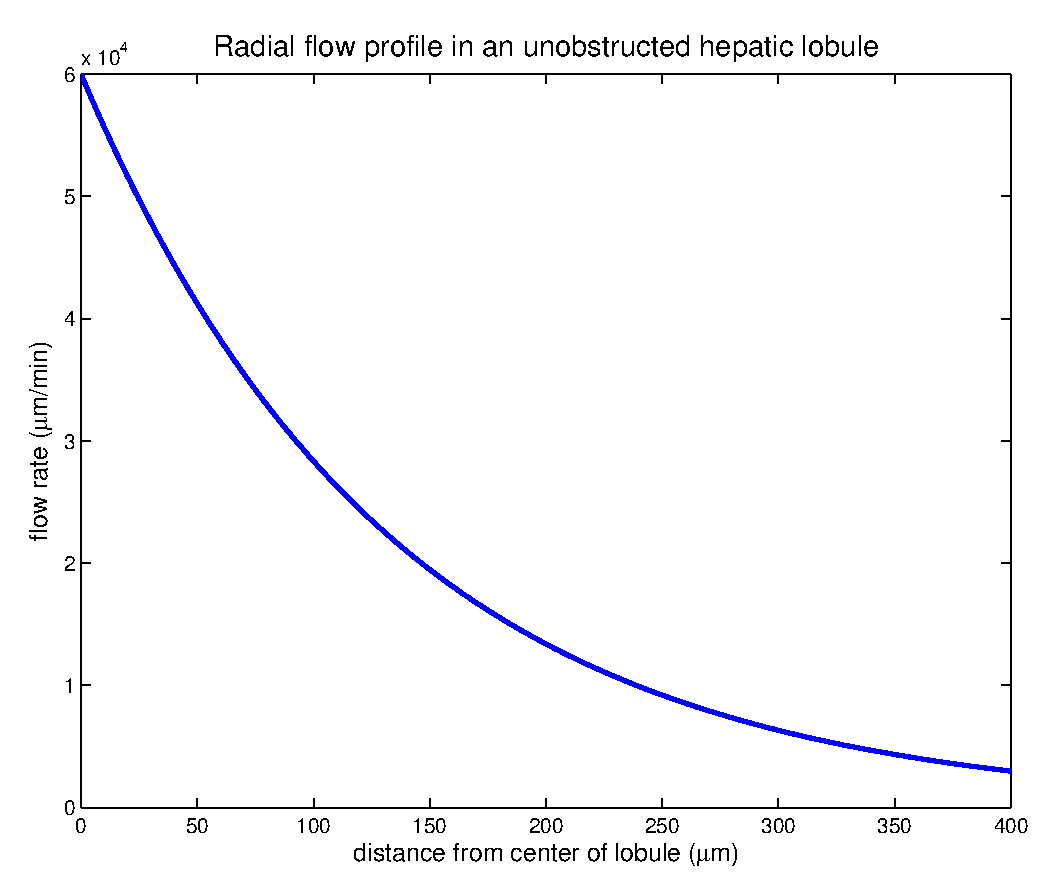
\includegraphics[width=6cm]{./figures/flow.eps}
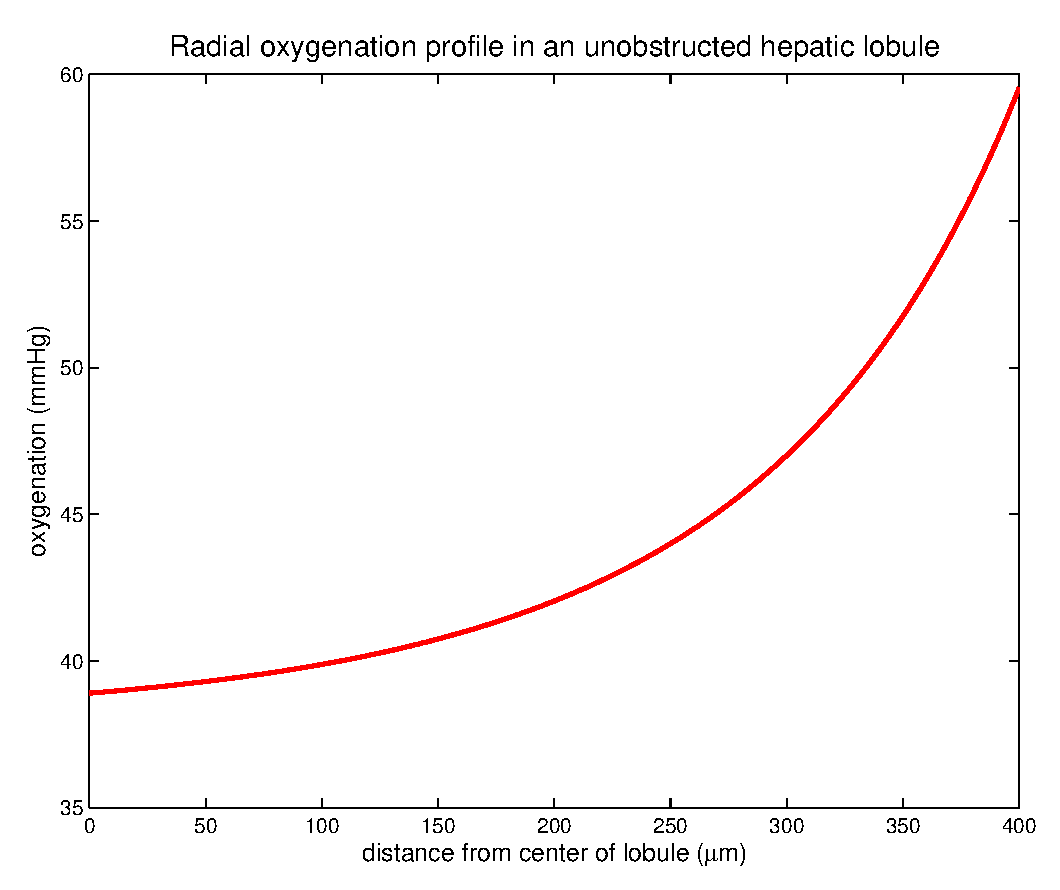
\includegraphics[width=6cm]{./figures/O2.eps}
\caption{Sample flow profile (left) and oxygenation profile (right) in a hepatic lobule, 
under the flow assumptions derived from the PVE model.}
\label{fig:radial_flow_oxygenation}
\end{figure}

\subsubsection{Approximating oxygen transport in large unobstructed liver tissues}
As described in Section \ref{sec:generate_liver}, we generated a large 1 cm$^2$ 
section of liver tissue with many hepatic lobules. Let 
$\braces{ \vec{x}_i }_{i=1}^n$ denote the centers of the hepatic lobules. 
We use the analytical solution from Section \ref{?} to approximate the 
quasi-steady oxygenation $\oxy$ in regions of intact, 
adevective flow-dominated tissue. If 
\beqa
r(\vec{x}) & = & \mathrm{min}\braces{ \norm{ \vec{x}_i -\vec{x}} }_{i=1}^n 
\eeqa
is the distance between $\vec{x}$ and the nearest central vein, 
then we approximate 
\beqa
\oxy(\vec{x}) & = & \sigma\left( r(\vec{x}) \right). 
\eeqa
Here, $\sigma$ is the radial oxygenation profile 
defined in Equation \ref{eqn:analytical_oxygen}. 

Note that this is equivalent to partitioning the 2-D tissue cross-section 
into a Voronoi mesh (with portal triads at the vertices (representing the 
flow source) and central veins in the centers) and assuming radial flow 
within each Voronoi polygon. See Fig. \ref{?}. 

\subsubsection{Integrating PVE insights: biotransport within tumors}
In Section \ref{?}, we saw that regardless of the relative (fluid) permeability 
of tumor tissue compared to normal liver parenchymal tissue, tumors with 
high interstitial fluid pressure (IFP) experience a near complete collapse of 
flow. High IFP is frequently reported in the literature for solid tumors, particularly larger ones with necrotic cores  
\cite{?}. 
% http://www.ncbi.nlm.nih.gov/pmc/articles/PMC1578509/
% Boucher, Y., Baxter, L. T. & Jain, R. K. Interstitial pressure gradients in tissue-isolated and subcutaneous tumors: implications for therapy. Cancer Res. 50, 4478–4484 (1990).
% http://journals.plos.org/plosone/article?id=10.1371%2Fjournal.pone.0140892
% http://www.maths.dundee.ac.uk/~chaplain/lowengrubetal_lymphangio_jtb.pdf
For simplicity, we shall assume that IFP is sufficiently high in all tumor tissue to disrupt flow, switching biotransport from advective-reactive to diffusive-reactive.  Thus, in tumor tissue, we model 
\beq
\frac{\partial \sigma}{\partial t}  =  
D \nabla^T \sigma - \lambda \sigma, 
\eeq
where $D = 10^5 \micron^2/\textrm{min}$ and $\lambda = 10 \textrm{ min}^{-1}$ as 
in \cite{?}. 

In Section \ref{?}, we examine the impact of relaxing this 
assumption, by assuming that IFP increases with distance from the nearest parenchymal agent, and that flow is eliminated (and hence biotransport is 
diffusive-reactive) beyond a fixed distance $L_\mathrm{cutoff}$ from 
functional parenchyme. 
\red{May need an additional necrosis mechanism}

\subsubsection{Tumor cell agents}
We model tumor cells using PhysiCell \cite{?} Version 1.0.0. We use the built-in ``live'' cell cycle model, 
with the default models of apoptosis and necrosis. Thus, each cell agent can be Live, Apoptotic, or Necrotic. 
Apoptosis is modeled as TME-independent, with a constant apoptotic death rate $d_A$ and a stochastic 
duration with mean $T_A$. We model necrosis as oxygen-dependent: cells enter the necrotic state if 
$\sigma < \sigma_N$, and then progress as described in \cite{?}. The rate of cell birth depends upon 
oxygenation as: 
\beq
b(\sigma)= \bar{b} \left( \frac{ \sigma -\sigma_N }{ \bar{\sigma} - \sigma_N } \right) 
\eeq
for reference values $\bar{b}$ and $\bar{\sigma}$. 

Tumor cells adhere to tumor and parenchymal agents, and push back 
with a ``repulsive'' restorative force as described in \cite{?}. 
We do not consider the impact of cell motility in this paper. 
Parameter values are given in Table \ref{tab:tumor_physicell_parameters}. 


\begin{table}
\begin{tabular}{cccc}
\textbf{Parameter} & \textbf{Biophysical meaning} & \textbf{Value} & \textbf{Reference}\\
\hline 
$R$ & cell radius & \\
$R_\mathrm{N}$ & nuclear radius & \\
$f_\mathrm{F}$ & cell fluid fraction & 0.75 \\
$\bar{b}$ & reference cell birth rate &  \\
$\sigma_N$ & threshold oxygen value for necrosis & 5 mmHg & \\
$T_A$ & mean duration of apoptosis & 8.6 hours & \\
$R_\mathrm{A}$ & maximum cell adhesion distance & $ 1.5 \: R$ \\
$C_\mathrm{cca}$ & cell-cell adhesion parameter &  \\
$C_\mathrm{ccr}$ & cell-cell repulsion parameter & \\
$\vdots$
\end{tabular}
\caption{Tumor cell parameters, using PhysiCell Version 1.0.0.}
\label{tab:tumor_physicell_parameters}
\end{table}

\subsubsection{Parenchymal agents}
Rather than model the individual hepatocytes and endothelial cells down to the 
sinusoidal microarchitectural scale, we model the overall parenchymal tissue 
as a collection of parenchymal agents, using the ``live'' cell cycle model, 
with the apoptotic death model (with stochastic duration). We assume that in 
the abscence of tumor cells, the tissue is in homeostasis with the birth rate 
and death rate both set to zero. 


% also cite Luigi's work 
%  https://hal.archives-ouvertes.fr/hal-00361051/file/final.pdf

The parenchymal agents exhange adhesive and ``repulsive'' forces with 
other parenchymal agents and tumor cells using the default mechanics 
model in PhysiCell. In addition, we extend our plasto-elastic model 
from \cite{?} to model parenchymal tissue deformation. To model 
elasticity, we assign each parenchymal agent $i$ 
(with position $\vec{x}_i$) a ``reference'' point $\vec{x}_{i,\mathrm{R}}$, 
and define the deformation $\vec{d}_i(t)$ by 
\beq
\vec{d}_i(t) = \vec{x}_{i,\mathrm{R}}(t) - \vec{x}_i(t).
\eeq
Where needed, define $d_i(t) = \norm{ \vec{d}_i(t) }$. 

After evolving the agent's position with the built-in PhysiCell mechanics model, 
(see \cite{?}) we further update the agent's position based upon 
the tissue elasticity: 
\beq
\frac{d}{dt} \vec{x}_i = r_\mathrm{E}
\vec{d}_i . 
\eeq
To model plastic reorganization of the parenchymal tissue, 
we evolve $\vec{x}_{i,\mathrm{R}}$: 
\beq
\frac{d}{dt}  \vec{x}_{i,\mathrm{R}} = -r_\mathrm{P} \vec{d}_i 
\eeq

\subsubsection{Integrating PVE insights: Constitutive relations for apoptosis}
In Section \ref{?}, we saw that there are significant fluid sheers and 
stress forces at the tumor-parenchymal interface. 
Such stresses are known to induce apoptosis \cite{?}. Thus, we will 
examine theree alternative constitutive relations for apoptosis of the 
parenchymal cells.

\paragraph{Apoptosis model 1: contact-based apoptosis (AM1)} If a parenchymal agent $i$ is 
in contact with a tumor cell, we set its state to apoptotic. 

\paragraph{Apoptosis model 2: deformation-based apoptosis (AM2)} If a parenchymal agent $i$ 
has $d_i(t) > d_\mathrm{max}$, we set its state to apoptotic. 

\paragraph{Apoptosis model 3: accumulated deformation-based apoptosis (AM3)} 
If a parenchymal agent $i$ has $\int_0^t d_i(s)\: ds > D_\mathrm{max}$, 
we set its state to apoptotic. 

\subsubsection{Numerical methods} We implemented the model 
in PhysiCell Version 1.0.0 \citep{?}, with BioFVM Version 1.1.14 \citep{ghaffarizadeh15_bioinformatics} to solve the oxygen biotransport equation. 
In regions of intact flow, we use ``Dirichlet nodes'' to impose the estimated 
to 

\vfill
\pagebreak` 




\subsubsection{Agents}
Describe tumor cell agents: substrate-driven growth, apoptosis, necrosis. Cell-cell adhesion, repulsion. Assume no 
motiltiy for now. Proliferation rate: 
\beq
a
\eeq

Apoptosis rate
\beq
a
\eeq

Necrosis rate
\beq
a
\eeq

Describe parenchyma agents. Rather than model individual hepatocytes, endothelial cells, model parenchyma as a collection 
of agents, diameter 30 $\micron$. Each parenchyma agent will follow regular adhesion-repulsion mechanics. In addition, we model 
mechanica interactions with underlying ECM. Each agent $i$ is attached to ECM at $\vec{x}_{i,\textrm{ECM}}$, and experiences 
an elastic force. Let $\vec{d}_i = \vec{x}_{i,\textrm{ECM}} - \vec{x}_i $, and let $d_i = \norm{ \vec{d}_i } - R_i$ denote 
the ellastic deformation. Then we use a force of the form 
\beq
\frac{d}{dt} \vec{x}_{i}(t) =r_\textrm{ECM} d_i  \frac{ \vec{d}_i }{ \norm{\vec{d}_i}} 
% \frac{d}{dt} \vec{x}_{i}(t) =r_\textrm{ECM} \Bigl(    \norm{ \vec{x}_{i,\textrm{ECM}} - \vec{x}_i } - R_i \Bigr) 
% \Bigl(    \norm{ \vec{x}_{i,\textrm{ECM}} - \vec{x}_i } - R_i \Bigr) 
% \frac{ \vec{x}_{i,\textrm{ECM}} - \vec{x}_i }{ \norm{ \vec{x}_{i,\textrm{ECM}} - \vec{x}_i } }. 
\eeq

To model plastic reorganization, we will evolve $\vec{x}_{i,\textrm{ECM}}$ by 
\beq
\frac{d}{dt} \vec{x}_{i,\textrm{ECM}} = r_\textrm{mech} \left( \vec{x}_{i} - \vec{x}_{i,\textrm{ECM}} \right)
\eeq

We shall not model proliferation in the parenchyma, instead assuming that it begins in a state of homeostasis. 
However, each agent (representnig a small section of tissue), will ahve a probabiltiy of apoptosing. 
IN this paper, we will investigate the following sub-models 

\paragraph{Model 1:} Parenchymal agents enter apoptotic state if 

\paragraph{Model 2:} Parenchymal agents enter apoptotic state if deformation $d_i$ exceeds a threshold 

\paragraph{Model 3:} Parenchymal agents enter apoptotic state if cumulative deformation 
$\int_0^t d_i(s)\: ds$ exceeds a threshold. 




\subsubsection{Integrating insights from the PVE model: mechanics}




% \subsubsection{Starting model assumptions}

\subsubsection{Parameter estimation}

\subsubsection{Numerical solution method} Here's where we say it's implemented in 
BioFVM Version (?) for PDE solvers, and PhysiCell Version (?) for agent-based model. 


\subsection{Results}

\subsubsection{Model results: dynamics for small tumor foci, no parenchyme apoptosis}
Use the assumptions from small tumors. (Good flow in tumors, so no diffusion, no gradients, parenchyme cells moved). 

\subsubsection{Model results: dynamics for small tumor foci, delayed parenchyme apoptosis} 
Use the assumptions from small tumors. (Good flow in tumors, so no diffusion, no gradients, parenchyme cells moved, 
assume the apoptose if moved too far). 

\subsubsection{Model results: dynamics for larger tumor foci, delayed parenchyme apoptosis} 
Use the assumptions from larger tumors. (Poor flow in tumors, diffusion, parenchyme cells moved, 
assume the apoptose if moved too far). 

\subsubsection{Model results: dynamics for larger tumor foci, immediate parenchyme apoptosis} 
Use the assumptions from larger tumors. (Poor flow in tumors, diffusion, parenchyme cells apoptose if near tumor cells). 





\section{Discussion and future directions \red{Paul, Jessica, Shannon}}
Recap of what we've learned. Does it mesh well with curently known stuff? Does it help explain clinical stuff? 

Future directions: critical to incorporate interstitial fluid flow with tumor cell volume changes. Likewise, need to drive porosity assumptions 
from tumor cell density. More direct, dynamical linking of codes. 

Add biochemical signaling, active tissue remodeling (rather than just deformation), advective terms in BioFVM to replace 
the cylindrical far-field assumptions. 

Follow-up. 3D is possible, but more insight on 3D lobular geometry, flow necessary. etc. 


\begin{acknowledgements}
PQ grant, BCRF grant, PSOC grant, support of CAMM, others?
\end{acknowledgements}

\section{Supplementary Materials \red{Paul, Jessica}}
\begin{enumerate}
\item 
Digital cell lines for tumor cells, parenchyma 
\item 
PhysiCell simulation source code
\item 
Simulation output data
\item 
Visualization routines 
\item 
Analysis scripts 
\item 
Anything else? 
\end{enumerate}

\bibliography{references}

\end{document}

